In the following section we present some high-level mockups of the system from the point of view of the user.
\subsection{Mobile Mockups}
These are some representations of how the mobile application should look like.\\ 
It should be noted that the finished product must follow the concept of these designs and not use the actual graphical elements here showcased, but a professional artist should be instead hired to design the interface given these guidelines.

\begin{figure}[h]
\centering
\begin{subfigure}{.5\textwidth}
  \centering
  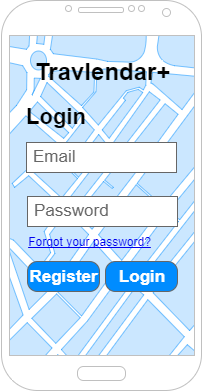
\includegraphics[height=.4\textheight, keepaspectratio=true]{Img/Login}
  \caption{Login interface}
\end{subfigure}%
\begin{subfigure}{.5\textwidth}
  \centering
  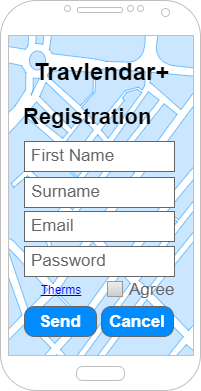
\includegraphics[height=.4\textheight, keepaspectratio=true]{Img/Registration}
  \caption{Registration interface}
\end{subfigure}
\caption{Login on the left (a) and Registration on the right (b)}
\end{figure}

\begin{figure}[h]
\centering
\begin{subfigure}{.5\textwidth}
  \centering
  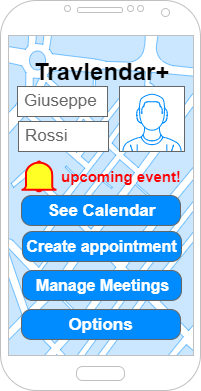
\includegraphics[height=.4\textheight, keepaspectratio=true]{Img/Home}
  \caption{Home page interface}
\end{subfigure}%
\begin{subfigure}{.5\textwidth}
  \centering
  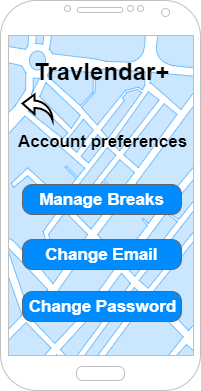
\includegraphics[height=.4\textheight, keepaspectratio=true]{Img/AccountOptions}
  \caption{Account Options interface}
\end{subfigure}
\caption{Home page on the left (a) and Account Options on the right (b)}
\end{figure}

\begin{figure}[h]
\centering
\begin{subfigure}{.5\textwidth}
  \centering
  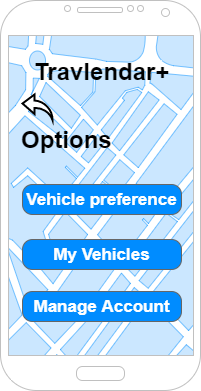
\includegraphics[height=.4\textheight, keepaspectratio=true]{Img/Options}
  \caption{Options interface}
\end{subfigure}%
\begin{subfigure}{.5\textwidth}
  \centering
  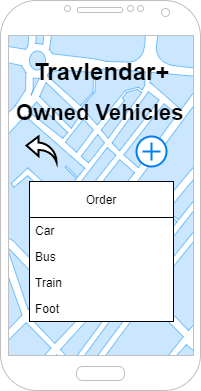
\includegraphics[height=.4\textheight, keepaspectratio=true]{Img/SpecifyMeans}
  \caption{Specify means of travel interface}
\end{subfigure}
\caption{Options on the left (a) and Specify means on the right (b)}
\end{figure}

\begin{figure}[h]
\centering
\begin{subfigure}{.5\textwidth}
  \centering
  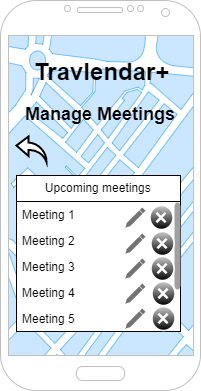
\includegraphics[height=.4\textheight, keepaspectratio=true]{Img/ManageMeeting}
  \caption{Manage Meeting interface}
\end{subfigure}%
\begin{subfigure}{.5\textwidth}
  \centering
  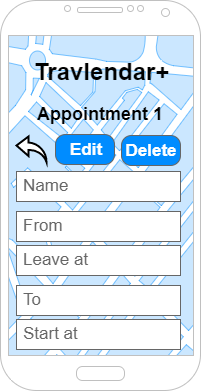
\includegraphics[height=.4\textheight, keepaspectratio=true]{Img/SelectedMeeting}
  \caption{Selected Meeting interface}
\end{subfigure}
\caption{Manage Meeting on the left (a) and Selected Meeting on the right (b)}
\end{figure}

\begin{figure}[h]
\centering
\begin{subfigure}{.5\textwidth}
  \centering
  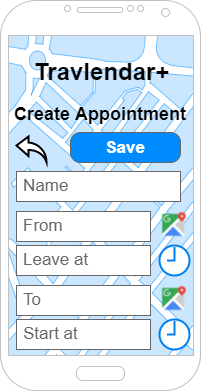
\includegraphics[height=.4\textheight, keepaspectratio=true]{Img/CreateAppointment}
  \caption{Create Appointment interface}
\end{subfigure}%
\begin{subfigure}{.5\textwidth}
  \centering
  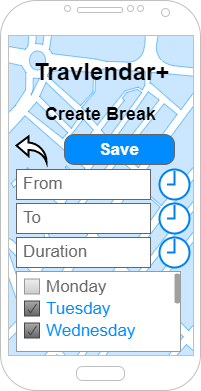
\includegraphics[height=.4\textheight, keepaspectratio=true]{Img/CreateBreak}
  \caption{Create Break interface}
\end{subfigure}
\caption{Create Appointment on the left (a) and Create Break on the right (b)}
\end{figure}
\clearpage
\subsection{Web Browser Mockups}
These are just a few examples of how the interface of the system should look like when looking at it via a web browser.\\
As it's quite clear it's the same design of the mobile application, the only difference is that it's reorganized for an aspect ratio more wide than high.\\
The designer in charge of the graphical elements should design the only one icon for action for both the mobile and the browser, and then making it as many times as it is needed in different dimensions and resolutions to adapt for different screen sizes.

\begin{figure}[h]
\centering
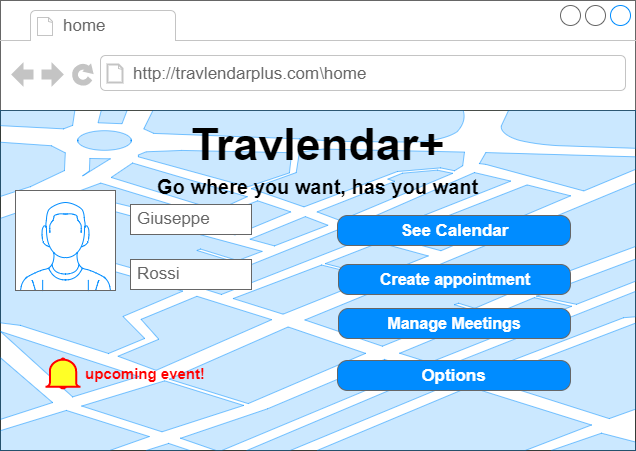
\includegraphics[height=.4\textheight, keepaspectratio=true]{Img/HomeDesktop}
  \caption{Home web browser interface}
\end{figure}

\begin{figure}[h]
\centering
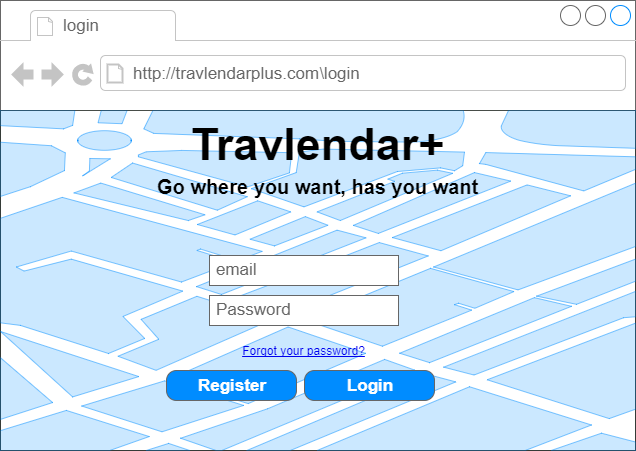
\includegraphics[height=.4\textheight, keepaspectratio=true]{Img/LoginDesktop}
  \caption{Login web browser interface}
\end{figure}

\begin{figure}[h]
\centering
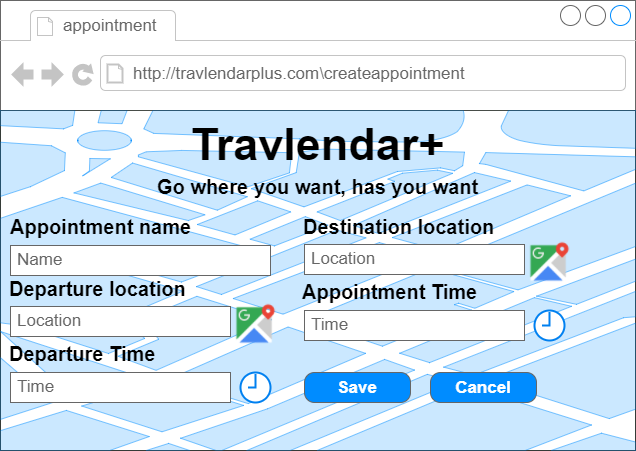
\includegraphics[height=.4\textheight, keepaspectratio=true]{Img/CreateAppointmentDesktop}
\caption{Create Appointment web browser interface}
\end{figure}


